%% LyX 2.3.4.2 created this file.  For more info, see http://www.lyx.org/.
%% Do not edit unless you really know what you are doing.
\documentclass{article}
\usepackage{amstext}
\usepackage{fontspec}
\setmainfont[Ligatures=TeX]{Jura}
\setsansfont[Ligatures=TeX]{Jura}
\setmonofont{Jura}
\usepackage{xcolor}
\usepackage{calc}
\usepackage{graphicx}
\usepackage{esint}

\makeatletter

%%%%%%%%%%%%%%%%%%%%%%%%%%%%%% LyX specific LaTeX commands.
%% Because html converters don't know tabularnewline
\providecommand{\tabularnewline}{\\}

\makeatother

\usepackage[serbianc]{babel}
\begin{document}
\title{Супер наслов}
\author{Ја, а ко би други?}
\maketitle
\begin{abstract}
Свашта, итд... Тако је то! Сада сам ти све рекао, шта више од тога!?
\end{abstract}

\section{Први}

Свашта ми је пало на памет па сам одлучио да почнем да пишем...\footnote{Кул}
\begin{quotation}
$\prod$и $\sum$ су супер слова.
\end{quotation}
\[
\int\sum\sqrt[3]{\text{џ}}
\]


\section{Други}

После одређеног времена сам одлучио да се ствари не морају мењати
драстично већ само у одређеној мери. Види страна број \pageref{sec:=000417=000430=00043A=000459=000443=000447=000430=00043A}.

$E=mc^{2}$\cite{key-1,key-2}
\begin{center}
$\begin{array}{cc}
1 & 0\\
0 & 1
\end{array}$
\par\end{center}

\begin{center}
{\fboxrule 1pt\fboxsep 5pt\fcolorbox{orange}{white}{\parbox[t]{0.3\columnwidth}{%
\begin{equation}
\alpha^{2}+\beta^{2}=\gamma^{2}\label{eq:=000421=000443=00043F=000435=000440}
\end{equation}
%
}}}
\par\end{center}

\newpage{}

\section{Трећи}

Могу још по нешто да додам.

\begin{figure}[h]
\begin{centering}
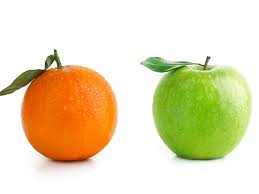
\includegraphics[scale=0.5]{first}
\par\end{centering}
\caption{Ово је баш супер сличица}

\end{figure}


\section{Закључак}

Све је било јако добро. Хвала.\label{sec:=000417=000430=00043A=000459=000443=000447=000430=00043A}

\begin{table}[h]
\begin{centering}
\begin{tabular}{|c|c|c|c|}
\hline 
а & б & в & г\tabularnewline
\hline 
\hline 
1 &  &  & \tabularnewline
\hline 
 & 1 &  & \tabularnewline
\hline 
 &  & 1 & \tabularnewline
\hline 
 &  &  & 1\tabularnewline
\hline 
\end{tabular}
\par\end{centering}
\caption{Супер табела}

\end{table}

\begin{thebibliography}{1}
\bibitem{key-1}Он

\bibitem{key-2}Ти
\end{thebibliography}

\end{document}
